\documentclass[12pt,a4paper]{article}

% Pacotes essenciais
\usepackage{karnaugh-map}
\usepackage[utf8]{inputenc}
\usepackage[T1]{fontenc}
\usepackage[portuguese]{babel}
\usepackage{amsmath, amsfonts, amssymb} % Matemática e lógica
\usepackage{graphicx} % Inserção de imagens (diagramas e esquemáticos)
\usepackage{booktabs} % Tabelas mais bonitas
\usepackage{multirow} % Mesclar linhas em tabelas
\usepackage{float} % Posicionamento rígido de figuras (H)
\usepackage{geometry}
\geometry{top=3cm, bottom=2cm, left=3cm, right=2cm} % Margens ABNT/Padrão
\usepackage{hyperref} % Links no sumário

\title{\textbf{Laboratório EEA-21 -- 2ª Experiência}\\ \large Circuitos Combinacionais: Multiplexadores, Decodificadores e Codificadores}
\author{Equipe: Marcello Ryaj e Matheus Levi/ Turma: Comp 28}
\date{\today}

\begin{document}

\maketitle
\tableofcontents
\newpage

% ---------------------------------------------------------
\section{Demultiplexador (DEMUX 1x4 com portas NOR)}

\subsection{Tabela Verdade e Expressões Booleanas}
Abaixo apresentamos a tabela verdade para o DEMUX 1x4. Considerando $En$ como a entrada de habilitação, $S_1$ e $S_0$ como chaves de seleção e $D$ como o dado de entrada.

\begin{table}[H]
    \centering
    \caption{Tabela Verdade do DEMUX 1x4}
    \begin{tabular}{cccc|cccc}
        \toprule
        \textbf{$En$} & \textbf{$S_1$} & \textbf{$S_0$} & \textbf{$D$} & \textbf{$Y_0$} & \textbf{$Y_1$} & \textbf{$Y_2$} & \textbf{$Y_3$} \\
        \midrule
        0             & X              & X              & X            & 0              & 0              & 0              & 0              \\
        1             & 0              & 0              & D            & D              & 0              & 0              & 0              \\
        1             & 0              & 1              & D            & 0              & D              & 0              & 0              \\
        1             & 1              & 0              & D            & 0              & 0              & D              & 0              \\
        1             & 1              & 1              & D            & 0              & 0              & 0              & D              \\
        \bottomrule
    \end{tabular}
\end{table}

As expressões booleanas na forma de Soma de Produtos (SOP) seriam:
\begin{align*}
    Y_0 & = En \cdot \overline{S_1} \cdot \overline{S_0} \cdot D \\
    Y_1 & = En \cdot \overline{S_1} \cdot S_0 \cdot D            \\
    Y_2 & = En \cdot S_1 \cdot \overline{S_0} \cdot D            \\
    Y_3 & = En \cdot S_1 \cdot S_0 \cdot D
\end{align*}

Para a implementação solicitada (apenas portas NOR), aplicamos o Teorema de De Morgan ($A \cdot B = \overline{\overline{A} + \overline{B}}$):
% Substitua pelas equações finais manipuladas
\begin{align*}
    Y_0 & = \overline{ \overline{En} + S_1 + S_0 + \overline{D} }                       \\
    Y_0 & = \overline{ \overline{En} + S_1 + S_0 + \overline{D} }                       \\
    Y_1 & = \overline{ \overline{En} + S_1 + \overline{S_0} + \overline{D} }            \\
    Y_2 & = \overline{ \overline{En} + \overline{S_1} + S_0 + \overline{D} }            \\
    Y_3 & = \overline{ \overline{En} + \overline{S_1} + \overline{S_0} + \overline{D} }
    % Adicione as demais aqui...
\end{align*}

\subsection{Diagrama Esquemático}
Para a obtenção do esquemático, as expressões originais foram convertidas para a base NOR invertendo duplamente a saída e aplicando De Morgan nas portas AND originais.

\begin{figure}[H]
    \centering
    % Substitua "nome_da_imagem.png" pelo arquivo do seu esquemático
    % \includegraphics[width=0.8\textwidth]{esquematico_4_1.png}
    \caption{Diagrama esquemático do DEMUX 1x4 (Portas NOR).}
\end{figure}

\subsection{Diagrama de Temporização}
\begin{figure}[H]
    \centering
    % \includegraphics[width=0.9\textwidth]{tempo_4_1.png}
    \caption{Simulação funcional (diagrama de temporização) do DEMUX 1x4.}
\end{figure}

% ---------------------------------------------------------


\section{Codificador (Gray para Binário 3 bits)}
\subsection{Código de Gray}
A partir do que foi fornecido, foi possível realizar a construção da tabela verdade, que é mostrado a seguir:

\begin{table}[!htb]
    \centering
    \begin{tabular}{|c|c|c|c|c|c|}
        \hline
        \textbf{Gray} & \textbf{B2} & \textbf{B1} & \textbf{B0} \\
        \hline
        000           & 0           & 0           & 0           \\
        001           & 0           & 0           & 1           \\
        011           & 0           & 1           & 0           \\
        010           & 0           & 1           & 1           \\
        110           & 1           & 0           & 0           \\
        111           & 1           & 0           & 1           \\
        101           & 1           & 1           & 0           \\
        100           & 1           & 1           & 1           \\
        \hline
    \end{tabular}
    \caption{Tabela verdade do conversor de código de Gray para binário.}
    \label{table:GrayTable}
\end{table}

A partir da tabela verdade, conseguimos ver que o bit mais significativo (B2) é igual ao bit mais significativo do código de Gray (G2). Além disso, foi realizado o mapa de Karnaugh para os bits B1 e B0, que são mostrados a seguir:

\begin{figure}[!ht]
\centering

\begin{karnaugh-map}[4][2][1][$G_2$][$G_1$][$G_0$]
\minterms{1, 2, 5, 6}
\implicant{1}{5}
\implicant{2}{6}

\end{karnaugh-map}

\caption{Mapa de Karnaugh para o Bit $B_1$ do binário puro}
\end{figure}

\begin{figure}[!ht]
\centering

\begin{karnaugh-map}[4][2][1][$G_2$][$G_1$][$G_0$]
\minterms{1, 2, 4, 7}
\end{karnaugh-map}

\caption{Mapa de Karnaugh para o Bit $B_0$ do binário puro}
\end{figure}

Dessa forma, percebe-se que o bit $B_1$ e o bit $B_0$ podem ser expressos como:

\begin{equation}
    B_1 = \overline{G_2}G_1 + G_2\overline{G_1} = G_1 \oplus G_2
\end{equation}

\begin{equation}
    B_0 = \bar{G_2}\bar{G_1}G_0 + \bar{G_2}G_1\bar{G_0} + G_2\bar{G_1}\bar{G_0} + G_2G_1G_0 = G_0 \oplus G_1 \oplus G_2
\end{equation}

Para o esquemático, foi utilizado o software Quartus, resultando no esquemático mostrado na Figura \ref{fig:CodGray}.

\begin{figure}[!ht]
    \centering
    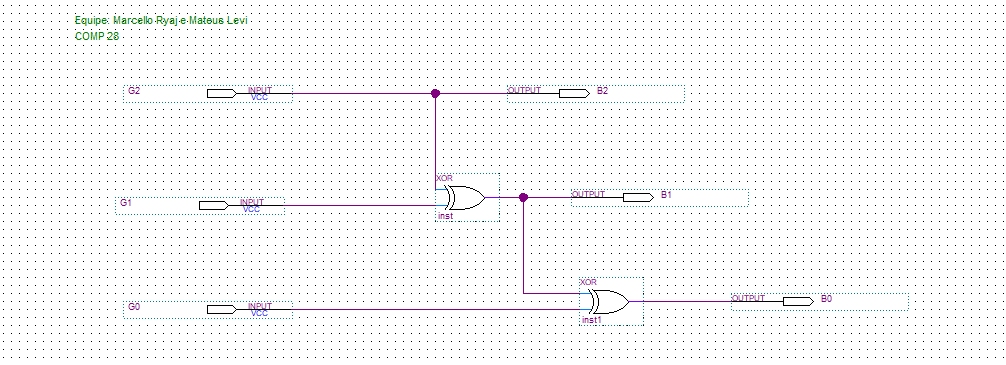
\includegraphics[width=0.8\textwidth]{fig/EsquematicoExercicio2.png}
    \caption{Esquemático do circuito para o Códificador Gray}
    \label{fig:CodGray}
\end{figure}

Após a realização do esquemático, foi possível realizar a simulação funcional, que é mostrada na Figura \ref{fig:SimulacaoExercicio2}.

\begin{figure}[!ht]
    \centering
    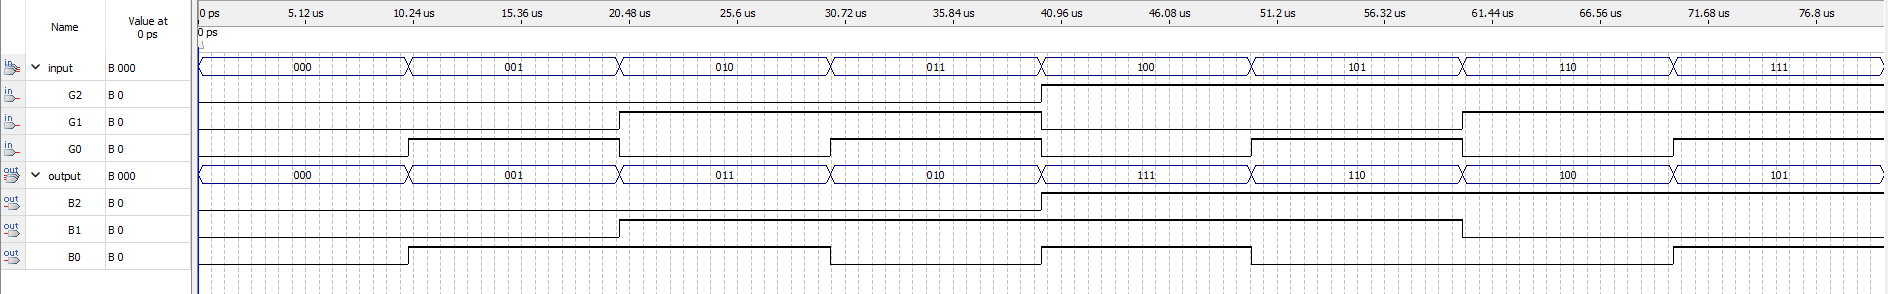
\includegraphics[width=1\textwidth]{fig/SimuExercicio2.png}
    \caption{Simulação funcional do circuito para o Códificador Gray}
    \label{fig:SimulacaoExercicio2}
\end{figure}

Comparando a simulação gerada com a tabela verdade produzida, é possível perceber que o circuito está funcionando corretamente, pois os bits de saída estão de acordo com o esperado para cada combinação de bits de entrada.






% ---------------------------------------------------------
\section{Decodificador 3x8}

\subsection{Tabela Verdade e Expressões Booleanas}

A tabela verdade de um decodificador 3x8 com entrada em binário puro ($A_2, A_1, A_0$) e entrada de habilitação ($En$) é apresentada a seguir. Quando $En = 0$, o decodificador está desabilitado e todas as saídas permanecem em nível baixo (0), independentemente dos valores de entrada. Quando $En = 1$, a combinação de entrada ativa exclusivamente a saída correspondente.

\begin{table}[H]
    \centering
    \caption{Tabela Verdade do Decodificador 3x8 com Enable}
    \begin{tabular}{cccc|cccccccc}
        \toprule
        \textbf{$En$} & \textbf{$A_2$} & \textbf{$A_1$} & \textbf{$A_0$} & \textbf{$Y_0$} & \textbf{$Y_1$} & \textbf{$Y_2$} & \textbf{$Y_3$} & \textbf{$Y_4$} & \textbf{$Y_5$} & \textbf{$Y_6$} & \textbf{$Y_7$} \\
        \midrule
        0             & X              & X              & X              & 0              & 0              & 0              & 0              & 0              & 0              & 0              & 0              \\
        1             & 0              & 0              & 0              & 1              & 0              & 0              & 0              & 0              & 0              & 0              & 0              \\
        1             & 0              & 0              & 1              & 0              & 1              & 0              & 0              & 0              & 0              & 0              & 0              \\
        1             & 0              & 1              & 0              & 0              & 0              & 1              & 0              & 0              & 0              & 0              & 0              \\
        1             & 0              & 1              & 1              & 0              & 0              & 0              & 1              & 0              & 0              & 0              & 0              \\
        1             & 1              & 0              & 0              & 0              & 0              & 0              & 0              & 1              & 0              & 0              & 0              \\
        1             & 1              & 0              & 1              & 0              & 0              & 0              & 0              & 0              & 1              & 0              & 0              \\
        1             & 1              & 1              & 0              & 0              & 0              & 0              & 0              & 0              & 0              & 1              & 0              \\
        1             & 1              & 1              & 1              & 0              & 0              & 0              & 0              & 0              & 0              & 0              & 1              \\
        \bottomrule
    \end{tabular}
\end{table}

A partir da tabela, extraímos as expressões booleanas simplificadas para cada saída. Como o decodificador só funciona quando habilitado, o termo $En$ deve estar presente (em nível lógico alto) em todas as equações, multiplicando os mintermos das entradas:

\begin{align*}
    Y_0 & = En \cdot \overline{A_2} \cdot \overline{A_1} \cdot \overline{A_0} \\
    Y_1 & = En \cdot \overline{A_2} \cdot \overline{A_1} \cdot A_0            \\
    Y_2 & = En \cdot \overline{A_2} \cdot A_1 \cdot \overline{A_0}            \\
    Y_3 & = En \cdot \overline{A_2} \cdot A_1 \cdot A_0                       \\
    Y_4 & = En \cdot A_2 \cdot \overline{A_1} \cdot \overline{A_0}            \\
    Y_5 & = En \cdot A_2 \cdot \overline{A_1} \cdot A_0                       \\
    Y_6 & = En \cdot A_2 \cdot A_1 \cdot \overline{A_0}                       \\
    Y_7 & = En \cdot A_2 \cdot A_1 \cdot A_0
\end{align*}

\subsection{Diagrama Esquemático}

\subsection{Diagrama de Temporização}

% ---------------------------------------------------------
\section{Codificador de Prioridade 4x2 (Produto de Somas)}

\subsection{Tabela Verdade e Expressões Booleanas}
A minimização foi realizada focando nos zeros (Maxtermos) para obter a forma de Produto de Somas (POS).

\subsection{Diagrama Esquemático}

\subsection{Diagrama de Temporização}

% ---------------------------------------------------------
\section{Codificador de Prioridade 8x3 (Expansão)}

\subsection{Expressões Booleanas e Esquemático do Bloco H}
A decomposição utiliza os módulos 4x2 projetados anteriormente. O Bloco H atua como a lógica combinacional de união.

\subsection{Diagrama de Temporização do Bloco H}

\subsection{Diagrama de Temporização do Dispositivo Completo}

\end{document}